\documentclass[../TDE1-E2.tex]{subfiles}%

\begin{document}
\section[s]"1"{Circuit simple}
\enonce{%
    On constitue un circuit électrique avec un générateur réel de tension $(E,r)$,
  entre les bornes duquel on branche une résistance $R$ réglable.
}%

\ifcorrige{%
  \begin{center}
    \begin{tcn}[width=.5\linewidth](data){Données}
      Générateur \underline{réel} $(E,r)$ de tension~: \smallbreak
      \begin{center}
        \includegraphics{circ_simple-a}
      \end{center}
    \end{tcn}
  \end{center}
}%

\QR{%
  Faire un schéma normalisé du circuit.
}{%
  \vspace{-15pt}
  \begin{tcbraster}[raster columns=3, raster equal height=rows]
    \begin{tcn}(ques){Résultat attendu}
      On demande un schéma \underline{normalisé}, autrement dit avec les
      conventions de schémas \textit{européennes}.
    \end{tcn}
    \begin{tcn}(tool)""{Outils}
      Générateur~:
      \includegraphics{circ_simple-b}
      \smallbreak
      Résistance~:\vspace{12pt}
      \includegraphics{circ_simple-c}
    \end{tcn}
    \begin{tcn}(appl)'r'{Application}
      On obtient~: \smallbreak
      \includegraphics{circ_simple-d}
    \end{tcn}
  \end{tcbraster}
}%

\QR{%
  Flécher les tensions et intensités, en respectant la convention pour
          chacun.
}{%
  \vspace{-15pt}
  \begin{tcbraster}[raster columns=2, raster equal height=rows]
    \begin{tcn}*(tool){Outils}
      Générateur convention générateur~: \smallbreak
      \vspace{-12pt}
      \begin{center}
        \includegraphics{circ_simple-e}
      \end{center}
      Résistance convention récepteur~: \smallbreak
      \vspace{-12pt}
      \begin{center}
        \includegraphics{circ_simple-f}
      \end{center}
    \end{tcn}
    \begin{tcn}(appl)'r'{Application}
      \begin{center}
        \includegraphics{circ_simple-g}
      \end{center}
    \end{tcn}
  \end{tcbraster}
}%

\QR{%
  Déterminer l'expression de l'intensité du courant qui circule dans le
          circuit.
}{%
  \vspace{-15pt}
  \begin{tcbraster}[raster columns=5, raster equal height=rows]
    \begin{tcn}[raster multicolumn=2](ques){Résultat attendu}
      À partir d'un circuit où on considère $E$, $r$ et $R$ comme des
      grandeurs connues, on cherche l'intensité $I$ qui parcourt la
      maille que l'on vient de tracer.
    \end{tcn}
    \begin{tcn}*[raster multicolumn=3](rema)"lrem"'r'{Remarque}
      Il y a deux outils qui seront utiles pour déterminer des grandeurs
      dans des circuits~: la \textbf{loi des mailles} et la \textbf{loi
      des nœuds}. À cela se rajoute la \textbf{loi d'Ohm} qui relie
      tension et intensité dans une résistance. Ces notions seront vues
      dans le chapitre suivant et donc décrites ultérieurement, on va
      ici utiliser la composition des tensions.
    \end{tcn}
  \end{tcbraster}
  \begin{tcbraster}[raster columns=3, raster equal height=rows]
    \begin{tcn}(tool){Outil}
      En nommant des points d'intérêt du circuit, ce qui est souvent
      conseillé, on va pouvoir utiliser la composition $U_\mathrm{AC} =
      U_\mathrm{AB} + U_\mathrm{BC}$ en respectant le sens des tensions
      pour obtenir une information supplémentaire sur le circuit.
      \smallbreak On rappelle que deux points sur un fil sont au même
      potentiel, et on peut donc les nommer de la même manière.
    \end{tcn}
    \begin{tcn}[raster multicolumn=2, sidebyside](appl)'r'{Application}
      \tcbsubtitle{\fatbox{Schéma}}
      \begin{center}
        \includegraphics{circ_simple-h}
      \end{center}
      \tcblower
      \tcbsubtitle{\fatbox{Calcul}}
      Ici on peut écrire
      \begin{align*}
        U_\mathrm{AB} + U_\mathrm{BC} + U_\mathrm{CA} & = U_\mathrm{AA} \\
        \Leftrightarrow -E + U_r + U_R                & = 0
      \end{align*}
      et avec la \textbf{loi d'Ohm}, i.e. $U_r = rI$ et $U_R = RI$~:
      \begin{equation*}
        (r+R)I = E\\
      \end{equation*}
      soit
      \begin{equation*}
        \boxed{I = \frac{E}{r+R}}
      \end{equation*}
    \end{tcn}
  \end{tcbraster}
}%

\QR{%
  Déterminer l'expression de la puissance absorbée par la résistance.
}{%
  \vspace{-15pt}
  \begin{tcbraster}[raster columns=2, raster equal height=rows]
    \begin{tcn}(tool){Outil}
      Pour un récepteur de tension $U$ traversé par l'intensité $I$ en
      convention récepteur, la puissance absorbée est \fbox{$P=UI$}.
    \end{tcn}
    \begin{tcn}(appl)'r'{Application}
      Ici, la tension aux bornes de $R$ est $U_R = RI$, avec $I$ l'intensité
      la traversant. On a donc
      \begin{equation*}
        \boxed{\Pc_R = RI^2 = \frac{RE^2}{(r+R)^2}}
      \end{equation*}
    \end{tcn}
  \end{tcbraster}
}%

\QR{%
  Tracer la courbe de $P$ en fonction de $R$, et montrer que cette
          courbe passe par un maximum. Déterminer les coordonnées du maximum.
}{%
  \vspace{-15pt}
  \begin{tcbraster}[raster columns=3, raster equal height=rows]
    \begin{tcn}(ques){Résultat attendu}
      On cherche à faire une étude de la fonction $P$ de variable $R$, comme
      on ferait l'étude de $f(x)$ en mathématiques.
    \end{tcn}
    \begin{tcn}[raster multicolumn=2](tool)'r'{Outils}
      Bon sens pour l'allure de la courbe, procédés de dérivation pour le
      maximum. D'une manière générale, on a besoin de~:
      \begin{itemize}
        \item Dérivation d'un produit~:
              \begin{equation*}
                \boxed{D[\textcolor{Purple!70}{u}
                      \textcolor{orange}{v}] =
                  \textcolor{brandeisblue}{u'}\textcolor{orange}{v} +
                  \textcolor{Red!70}{v'}\textcolor{Purple!70}{u}}
              \end{equation*}
        \item Dérivation d'une fonction $u$ élevée à une puissance
          $\alpha$ ~:
              \begin{equation*}
                \boxed{D[\textcolor{Purple}{u}^
                {\textcolor{ForestGreen}{\alpha}}] =
              \textcolor{ForestGreen}{\alpha}
            \textcolor{brandeisblue}{u'}
          \textcolor{Purple}{u}^{\textcolor{Goldenrod}{\alpha-1}}}
              \end{equation*}
      \end{itemize}
    \end{tcn}
  \end{tcbraster}
  \vfill
  \begin{tcn}[breakable, sidebyside,
    righthand width=.5\linewidth](appl){Application}
    \tcbsubtitle{\fatbox{Tracé}}
    \hspace{-12pt}
    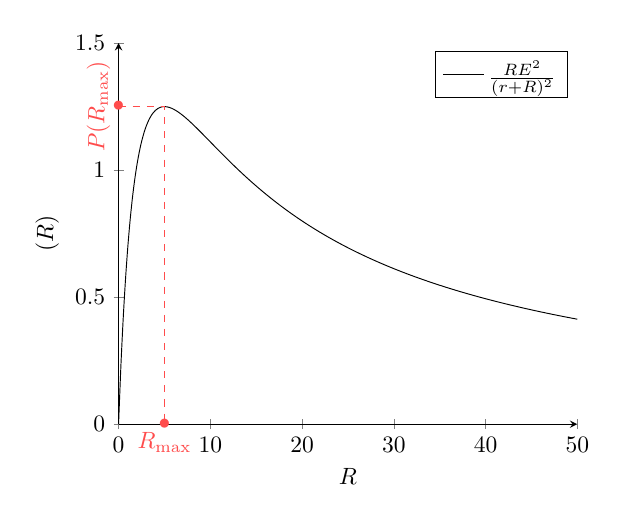
\begin{tikzpicture}[scale=0.85]
      \def\E{5}
      \def\r{5}
      \begin{axis}[
          axis lines=left,
          xmin=0, xmax=50,
          ymin=0, ymax=1.5,
          xlabel=$R$, ylabel=$\Pc(R)$,
          clip=false]
        \addplot[
          domain=0:50,
          samples=200,
          smooth]
        {x*\E^2/(\r+x)^2};
        \addlegendentry{$\frac{RE^2}{(r+R)^2}$}
        \draw[dashed, Red!70]
        (0,1.25) node {$\bullet$} node [above, rotate=90]
        {$P(R_\mathrm{max})$} --++
        (5,0) --++
        (0,-1.25) node {$\bullet$} node[below] {$R_\mathrm{max}$};
      \end{axis}
    \end{tikzpicture}
    \tcblower
    \tcbsubtitle{\fatbox{Calcul}}
    Soit
    \begin{itemize}
      \item $ \textcolor{orange}{v(R) = R}
              \Longrightarrow
              \textcolor{Red}{v'(R) = 1}$
      \item $ \textcolor{Purple}{u(R) = r+R}
              \Longrightarrow
              \textcolor{brandeisblue}{u'(R)=1}$
    \end{itemize}
    Ainsi
    \[
      \textcolor{Purple}{u(R)}^{\textcolor{ForestGreen}{{-2}}} =
      \frac{\textcolor{ForestGreen}{1}}
      {\textcolor{Purple}{(r+R)}^{\textcolor{ForestGreen}{2}}}
      \Rightarrow
      D[\textcolor{Purple}{u(R)}^{\textcolor{ForestGreen}{{-2}}}] =
      \frac{\textcolor{ForestGreen}{-2}
      \times\textcolor{brandeisblue}{1}}
      {\textcolor{Purple}{(r+R)}^{\textcolor{Goldenrod}{3}}}
    \]
    \bigbreak
    Et donc,
    \begin{align*}
      \Pc'(R) & = \frac{\textcolor{ForestGreen}{-2}}
      {\textcolor{Purple}{(r+R)}^{\textcolor{Goldenrod}{3}}}
      \times \textcolor{orange}{R} + \textcolor{Red}{1}\times
      \frac{\textcolor{ForestGreen}{1}}
      {\textcolor{Purple}{(r+R)}^{\textcolor{ForestGreen}{2}}} \\
      \Pc'(R) & = \frac{-2R}{(r+R)^3} + \frac{r+R}{(r+R)^3}
    \end{align*}
    Ainsi
    \begin{equation*}
      \boxed{\Pc'(R) = \frac{r-R}{(r+R)^3}}
    \end{equation*}
    Et donc
    \begin{equation*}
      \Pc'(R_\mathrm{max}) = 0 \Longrightarrow
      \textcolor{Red!70}{\boxed{R_\mathrm{max} = r}}
    \end{equation*}
    Avec
    \begin{equation*}
      \textcolor{Red!70}{\boxed{\Pc(R_\mathrm{max}) = \frac{E^2}{4r}}}
    \end{equation*}
  \end{tcn}
}%

\end{document}
